\chapter{Should Machines Decide? Lindley's Challenge}
\label{ch:lindleyai}

\section{The challenge restated}

Chapter~\ref{ch:why} introduced Lindley's challenge: if the task of a court is to combine probabilities and utilities coherently, then the task is a computation, and a machine could perform it at least as well as a person, leaving to people the statement of utilities and the supply of evidence. Lindley did not live to see large language models, but he saw enough of computing to understand that the question would become practical. It has. This chapter asks how artificial intelligence is already changing court decisions, how it is likely to change them over the next decade, and what a Bayesian view implies about how it should be governed.\index{Lindley's challenge}\index{artificial intelligence!in courts}

We begin with what is already happening, then describe ten channels through which AI will change decisions, then examine the fairness questions raised by risk assessment, and close with Lindley's own answer, restated as a set of requirements.

\section{What machines already do}

\subsection{Risk assessment}

Many American jurisdictions use actuarial risk assessment tools to inform decisions on pretrial release, sentencing and parole. Such tools estimate the probability that a person will fail to appear or be rearrested, using criminal history, age and other factors. In \emph{State v Loomis} the Wisconsin Supreme Court held in 2016 that a sentencing court's consideration of a proprietary risk score did not violate due process, provided the score was not determinative and the court was warned of its limitations, including that its methodology was a trade secret and that it had been criticised for treating groups differently \citep{loomis2016}. The same year, a ProPublica investigation of one such tool reported that black defendants who did not reoffend were more likely than white defendants who did not reoffend to have been labelled high risk \citep{angwin2016}. The debate that followed, discussed below, produced important results about what fairness can and cannot mean for a probabilistic predictor.\index{risk assessment}\index{State v Loomis}

\subsection{Prediction of decisions}

Researchers have built models that predict the outcomes of court decisions from case features or texts. Aletras and colleagues predicted decisions of the European Court of Human Rights from the text of its judgments' factual sections with accuracy well above chance \citep{aletras2016}. Katz, Bommarito and Blackman built a model that predicted decisions of the United States Supreme Court over two centuries with accuracy around seventy per cent \citep{katz2017}. Kleinberg, Lakkaraju, Leskovec, Ludwig and Mullainathan compared machine predictions of pretrial misconduct with the bail decisions of judges in New York City and estimated that a machine learning rule could reduce crime substantially at the same detention rate, or reduce detention substantially at the same crime rate \citep{kleinberg2018}. Their study confronted the selective labels problem: outcomes are observed only for defendants judges released, so the model's predictions for those detained cannot be checked directly. They used the quasi random assignment of cases to judges with different release rates to address it. The problem is one of missing data, and its careful treatment is what made the study credible.

\subsection{Documents and discovery}

In large civil cases, the review of documents for disclosure is now routinely assisted by machine learning. In \emph{Da Silva Moore v Publicis Groupe} a federal magistrate judge in New York approved the use of technology assisted review in 2012 \citep{dasilva2012}, and in \emph{Pyrrho Investments v MWB Property} the English High Court approved predictive coding for disclosure in 2016 \citep{pyrrho2016}. The courts reasoned that the method's recall and precision could be measured and were at least as good as human review at far lower cost. This is an argument from measured error rates, and it has been accepted.

\subsection{Language models}

Since 2023, lawyers and litigants have used large language models to draft submissions, with mixed results. In \emph{Mata v Avianca}, a federal judge in New York sanctioned lawyers who had filed a brief citing cases that did not exist, invented by a language model \citep{mata2023}. In 2025 the Divisional Court in England, in \emph{Ayinde v London Borough of Haringey}, warned that lawyers who put fictitious citations before the court face serious professional consequences, and set out the duties of lawyers who use such tools \citep{ayinde2025}. Judicial guidance in England and Wales, first issued in December 2023 and updated since, accepts that judges may use AI tools to assist with some tasks, while warning against reliance on them for legal research or analysis and insisting that they cannot replace the judge's direct engagement with the evidence \citep{judguidance2025}. The European Union's AI Act classifies AI systems intended to assist judicial authorities in researching and interpreting facts and law as high risk, subject to requirements of risk management, data quality, transparency and human oversight \citep{euaiact2024}.

\subsection{Online courts}

Richard Susskind has argued for online courts that resolve disputes without hearings, with judges deciding on written submissions supplemented by online tools that help parties understand their rights and options \citep{susskind2019}. British Columbia's Civil Resolution Tribunal, which began operating in July 2016 with strata property claims and took small claims from June 2017, handles such disputes largely online. Such systems are not yet machine judges, but they move many steps of dispute resolution to software.

\section{Ten ways AI will change court decisions}

We now describe the channels through which AI is changing and will change the decisions courts make. Some are already visible; others are plausible extrapolations. Each can be analysed with the tools of this book.

\subsection{Triage and scheduling}

Courts under load, as Chapter~\ref{ch:india} showed, face a scheduling problem. Machine learning can estimate the time a case will take, the probability of settlement or adjournment, and the cost of delay to the parties, and so support priority rules such as the $c\mu$ rule. This changes decisions indirectly, by changing which cases are heard and when, and directly, since delay itself determines outcomes for detained defendants and for parties whose claims lose value. The Bayesian requirement is that the estimates be calibrated and that their errors not fall systematically on particular groups.

\subsection{Drafting and summarising}

Language models already summarise bundles, draft chronologies and propose orders. For judges with heavy caseloads, this may be the most immediate change. The risk is that the summary shapes the decision: a judge who reads the machine's account of the evidence may not notice what it omitted. The Bayesian discipline is to treat the summary as a signal with an error rate, and to require that summaries be checked against sources, as the courts in \emph{Mata} and \emph{Ayinde} required for citations.

\subsection{Evidence analysis}

Machines will analyse more of the evidence: documents, communications, financial records, video and audio. Technology assisted review is the first example. Network analysis of communications, as in the organised crime cases of Chapter~\ref{ch:gould}, and anomaly detection in financial records, as in the bankruptcy cases of Chapter~\ref{ch:bankruptcy}, will become routine. Each produces outputs with error rates that must be reported as likelihood ratios, not as conclusions. A machine that flags a transaction as suspicious provides evidence whose weight depends on the machine's true and false positive rates, and whose effect on the posterior depends also on the base rate of suspicious transactions, exactly as for the polygraph in Chapter~\ref{ch:fienberg}.

\subsection{The authenticity of evidence}

AI also changes the evidence itself. Generative models can produce realistic images, audio and video of events that did not happen. This changes the likelihood ratio of every recording. Before such tools, a video showing the defendant at the scene usually had a large likelihood ratio, because the probability of such a video existing if he was not there was small. Now that probability includes the probability of fabrication, which is no longer negligible. By the logic of equation \eqref{eq:lowtemplate}, the likelihood ratio of a recording is bounded by the reciprocal of the fabrication probability. Courts will need methods of authentication, such as cryptographic provenance, and expert evidence on the probability of fabrication. There is also a converse effect, sometimes called the liar's dividend: a party confronted with genuine evidence can claim it is fabricated, and the claim is more plausible than it used to be. Both effects push courts toward evidence with verifiable chains of custody.\index{deepfakes}

\subsection{Prediction and settlement}

If parties can predict outcomes more accurately, the Priest and Klein model of Chapter~\ref{ch:becker} predicts that more disputes will settle, since disagreement about the outcome is what drives trials. The cases that remain will be those where prediction is genuinely hard: novel legal questions, close factual disputes, and, in other models, cases where one party has private information. Courts will see fewer easy cases and more hard ones. This changes the work of judges and the development of law. Precedent will be generated by a sample even more selected toward the frontier. A Bayesian legal system would track this selection and correct for it when learning from decided cases.

\subsection{Decision support with probabilities}

Judges will increasingly receive probabilities: of reoffending, of a party's success, of a document's authenticity, of a contamination event. How they use them matters. Experimental evidence suggests that people underuse algorithmic advice after seeing it err \citep{dietvorst2015}, and the literature on automation bias suggests that people can also accept machine outputs without scrutiny. The Bayesian framework says how a probability should be used: as an input to an expected utility calculation, weighed against other evidence according to its likelihood ratio and reliability. Training judges in this use is as important as building the tools.

\subsection{Consistency}

Machines can detect inconsistency. A system that compares a judge's sentence with those given in similar cases, or an appellate court's ruling with its precedents, can flag outliers for review. Inconsistency is a form of noise in the sense of Kahneman, Sibony and Sunstein: unwanted variability in judgments that should be the same \citep{kahneman2021}. Studies of asylum decisions have found large differences between adjudicators on similar cases \citep{ramji2007}, and studies of sentencing report similar disparities. Reducing noise is valuable, but it raises the question France answered in its 2019 ban on judge analytics (Chapter~\ref{ch:commoncivil}): should the performance of individual judges be measured? A Bayesian view is that noise is a cost, measurable as the expected loss from inconsistent decisions, and that measuring it is the first step to reducing it.

\subsection{Access to justice}

Most people with legal problems never see a lawyer or a court. Machine guidance, through online tools that explain rights, prepare documents and suggest outcomes, may bring legal information to many who now go without. This could be the largest change of all, and the hardest to see in court statistics, since its effect is on disputes that never reach court. The risk is that poor quality guidance misleads people about their rights; the remedy is evaluation, with randomised trials where possible, of whether guidance improves outcomes.

\subsection{Verification and transparency}

As Chapter~\ref{ch:lean} argued, formal verification can certify the logical and arithmetical parts of legal reasoning. Combined with language models that propose arguments, it could make routine decisions, such as the computation of benefits or the application of sentencing guidelines, faster and checkable. This changes decisions by removing a class of error.

\subsection{The role of the judge}

Taken together, these changes shift the judge's role toward the parts of decision that machines cannot perform: finding contested facts, interpreting open textured law, weighing values and taking responsibility. Lindley's division, machines compute and people supply utilities, describes the direction of change, though the boundary will move as machines improve.

\section{Fairness and calibration}

\subsection{The impossibility results}

The debate over risk assessment produced a mathematical result with direct legal consequences. A risk score can be calibrated, meaning that among people given a score of $s$, a fraction $s$ reoffend, within each group. It can also be balanced: those who go on to reoffend can receive the same average score in each group, and so can those who do not. Kleinberg, Mullainathan and Raghavan showed that when base rates of reoffending differ between groups, no score other than a perfect predictor can be calibrated within groups and balanced for both the positive and the negative class \citep{kleinberg2017}. For a yes or no classification the corresponding result, due to Chouldechova, is that equal positive predictive values across groups with different base rates $p$ force the error rates apart, by the identity $\mathrm{FPR}=\frac{p}{1-p}\,\frac{1-\mathrm{PPV}}{\mathrm{PPV}}\,(1-\mathrm{FNR})$: the false positive rate or the false negative rate must differ, unless the positive predictive value is zero or one \citep{chouldechova2017}.\index{calibration}\index{fairness}

\begin{figure}[t]
\centering
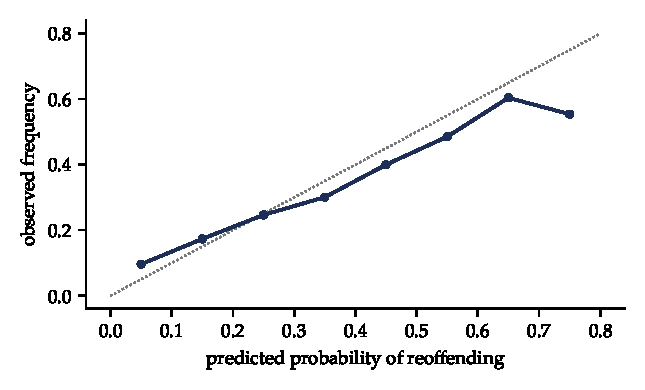
\includegraphics[width=\linewidth]{fig_calibration}
\caption{A calibration plot for a simulated risk tool. Predicted probabilities are grouped into bins, and the observed frequency of the outcome in each bin is plotted against the average prediction. A well calibrated tool lies on the diagonal.}
\label{fig:calibration}
\end{figure}

\subsection{The Bayesian view}

From a Bayesian standpoint, calibration is the natural requirement for a probability that will be used in a decision. A decision maker who maximises expected utility needs the probability that the event will occur, and only a calibrated score supplies it. Figure~\ref{fig:calibration} shows a calibration check. Error rate parity is a property of a decision rule, not of a probability. If society wants to move the error rates across groups, it can change the decision thresholds by group while keeping the probabilities calibrated, which is a choice about utilities. One threshold per group can in general equalise only one error rate, not both, and equalising both would need randomisation. Group-specific thresholds also raise legal problems: a threshold that depends on race is an explicit racial classification, which in the United States invites equal protection scrutiny and in England and Wales claims of direct discrimination under the Equality Act 2010. Separating the probability from the decision, as Lindley would, clarifies what the fairness debate is about: whether the utilities used in a decision should differ across groups, a question of values as much as of statistics, and one the law constrains.

There is a further point. A calibrated score may be calibrated on biased data. If arrests, not offences, are the outcome, and if policing is more intensive in some neighbourhoods, then the score predicts arrests, and its calibration reproduces the bias of policing. The Bayesian remedy is to model the measurement process, the relation between offences and arrests, explicitly, rather than to treat the observed outcome as the truth. This is the same lesson as the selective labels problem: a model is only as good as its account of how its data were generated.

\section{Lindley's answer}

We can now state what we take to be Lindley's answer to his own challenge, translated into requirements for machines in courts.

\begin{keybox}
Requirements for a Bayesian machine in court.
\begin{enumerate}[label=\arabic*.]
\item Probabilities, not verdicts. The machine reports calibrated probabilities with stated uncertainty, not bare conclusions.
\item Explicit utilities. The losses used in any decision rule are stated, set by legislatures or courts, and open to challenge.
\item Separation. The probability model and the decision rule are separate, so that each can be examined and changed independently.
\item Calibration checks. The machine's probabilities are tested for calibration, overall and within groups, on data from the population where it is used.
\item A model of the data. The machine's account of how its training data were generated, including selection and measurement, is documented.
\item Verifiable computation. The arithmetic from inputs to outputs can be checked by the parties.
\item Contestability. A party can challenge any input, and the effect of the challenge on the output is shown.
\item Human responsibility. A person, identified and accountable, adopts the decision and gives reasons.
\end{enumerate}
\end{keybox}

These requirements are demanding, and few current systems meet them. The proprietary risk tool in \emph{Loomis} met almost none: its model was secret, its utilities implicit, and its fairness disputed. ProPublica challenged its error rates across race, while its developer \citep{dieterich2016} and Flores, Bechtel and Lowenkamp argued that it was calibrated and satisfied predictive parity \citep{flores2016}. A tool built to these requirements would be more transparent than most human decision making, which is the point Lindley would have made. A judge does not state her probabilities or utilities, and her calibration is rarely checked. The question is not whether machines are perfect but whether a machine held to these standards, and overseen by a judge, would make better decisions than a judge alone. For many routine decisions, we think the answer is yes. For the hardest decisions, those that turn on contested facts, open texture and values, the machine can inform but should not decide.

Lindley's own view, as we understand it, was characteristically blunt: coherence is coherence, whoever achieves it. A court that reasons incoherently does injustice whether it is staffed by people or by machines. The opportunity that AI offers is to make the structure of legal reasoning explicit, so that incoherence can be seen and corrected. The danger is that it will be used to hide the structure further, behind proprietary models and fluent text. Which of these happens depends on choices that lawyers, judges and legislators are making now.

\section*{Notes and Questions}
\addcontentsline{toc}{section}{Notes and Questions}
\begin{enumerate}[label=\arabic*.]
\item Read \emph{State v Loomis}. Which of the eight requirements did the risk tool satisfy? What would the court have had to require to satisfy the rest?
\item Show that if two groups have different base rates and a yes or no classification has the same positive predictive value and the same false negative rate in each group, then its false positive rates differ unless its positive predictive value is zero or one. (Hint: write the false positive rate in terms of the base rate, the positive predictive value and the false negative rate.)
\item A video purports to show the defendant at the scene. An expert estimates that, if the defendant was not at the scene, the probability that a fabricated video of this quality would exist is one in a thousand. What is the maximum likelihood ratio of the video? How should the court proceed if authenticity is disputed?
\item Kleinberg and colleagues faced the selective labels problem. Explain it, and explain how quasi random assignment of judges helps.
\item Using the Priest and Klein model, predict how better outcome prediction would change the composition of cases reaching trial and the plaintiff win rate.
\item Draft a practice direction for the use of language models by judges in your jurisdiction. Which of the ten channels in this chapter does it address?
\item Should France's ban on analytics about individual judges be adopted elsewhere? Argue both sides in terms of noise, value of information and judicial independence.
\end{enumerate}

\section*{Further reading}
Kleinberg and colleagues on bail \citep{kleinberg2018}; Chouldechova \citep{chouldechova2017} and Kleinberg, Mullainathan and Raghavan \citep{kleinberg2017} on fairness; Susskind on online courts \citep{susskind2019}; Kahneman, Sibony and Sunstein on noise \citep{kahneman2021}.
